
\documentclass[a4paper, 14pt]{extreport}
\usepackage{scrextend}
\usepackage{amsmath}
\usepackage[a4paper, left = 20mm, right = 20mm, top = 13mm, bottom = 15mm]{geometry}
\usepackage[unicode]{hyperref}
\urlstyle{same}
\usepackage{graphicx}
\graphicspath{./}
\usepackage[utf8]{inputenc}
\usepackage[russian]{babel}
    

\title{{\textbf{Введение в Численные Методы\\ Аналитический отчёт по практическому заданию}}}
\author{Выполнила студентка 208 группы ВМК МГУ\\ Мазур Анастасия Вадимовна}
\date{}

\begin{document}
\maketitle

\begin{center}
    Var 2 ex 1
\end{center}

\section*{Математическая постановка задачи}

Функция $f(x)$  задана таблично на отрезке [0, a] в точках $x_{i}$, $x_{i} = ih$, \\
$i = 0, 1, ..., n, h = a / n$

\begin{itemize}
\item{Построить интерполяционный многочлен по точкам $x$.} 
\item{Приблизить функцию по методу наименьших квадратов  полиномом   заданной степени $n$, $n < 9$. Оценить погрешность.} 
\item{Результаты сравнить.}
\end{itemize}

\noindent{Отрезок $[0, 2]$}\\
Таблица значений функции в точках: \\ \\
\indent\begin{tabular}{|c|c|c|} 
    \hline\( i \) & \( x \) & \( f(x) \) \\ 
    \hline 0 & 0 & 0 \\ 
    \hline 1 & \( 0.2 \) & \( 0.006732 \) \\ 
    \hline 2 & \( 0.4 \) & \( 0.058195 \) \\ 
    \hline 3 & \( 0.6 \) & \( 0.030482 \) \\ 
    \hline 4 & \( 0.8 \) & \( 0.387483 \) \\ 
    \hline 5 & \( 1 \) & \( 0.958924 \) \\ 
    \hline 6 & \( 1.2 \) & \( 0.48283 \) \\
    \hline 7 & \( 1.4 \) & \( 1.802771 \) \\ 
    \hline 8 & \( 1.6 \) & \( 4.052411 \) \\
    \hline 9 & \( 1.8 \) & \( 2.403475 \) \\
    \hline 10 & \( 2 \) & \( 4.352169 \) \\
    \hline
\end{tabular}

\section*{Используемые алгоритмы, формулы и условия применимости}
\subsection*{Построение интерполяционного многочлена \\ в форме Лагранжа}
\indent{Чтобы интерполировать функцию построим полином в форме Лагранжа. \\ Искомый полином $P_{n}(x)$ будет иметь следующий вид:}

$$P_{n}(x) = \sum_{i = 0}^{n} f\left(x_{i}\right) Q_{n, i}(x),$$
где $Q_{n, i}(x)$ - полиномы степени $n$, "ориентированные" на точки $x_{i}$ \\ в том смысле, что
$$
Q_{n, i}(x)=\left\{\begin{array}{l}0, x=x_{j}, \; \; \forall j \neq i \\ 1, x=x_{i}\end{array}\right. $$

{Полиномы имееют вид: $$Q_{n, i}(x)=\prod_{j=0 \atop j \neq i}^{j=n} \frac{\left(x-x_{j}\right)}{\left(x_{i}-x_{j}\right)}$$}
или в нашем случае, когда $x_{i} = ih$, то есть известны значения в точках, расстояние между которыми фиксировано, то выражение можно упростить до следующей записи:
$$	
Q_{n, i}(x)=h^{-n} \cdot \prod_{j=0 \atop j \neq i}^{n} \frac{(x-j h)}{(i-j)}
$$

Учитывая, что полином в форме Лагранжа $P_{n}(x)$ представляет собой линейную комбинацию алгебраических уравнений $f(x_{i})Q_{n, i}(x), Q_{n, i}(x)$ - полиному степени n, можно утверждать, что $P_{n}(x)$ будет иметь степень не более $n$.
\\ \\
\indent{Данные формулы будут далее использоваться в программной реализации.}
\subsection*{Приближение функции методом наименьших квадратов}

\indentВ методе наименьших квадратов аппроксимирующая функция $y(x)$ ищется в виде следующей суммы:
$$F(x)=\sum_{k=0}^{m} a_{k} \varphi_{k}(x), \; \; m<n$$

{В каждой точке сетки $x_{i}$ можно подсчитать погрешность:}
$$\delta_{i}=y_{i}-F\left(x_{i}\right)=y_{i}-\sum_{k=0}^{m} a_{k} \varphi_{k}\left(x_{i}\right), \; \; \; i=0,1,2, \ldots, n$$

Сумма квадратов этих величин называется суммарной квадратичной погрешностью
$$J=\sum_{i=0}^{n} \delta_{i}^{n}=\sum_{i=0}^{n}\left(y_{i}-\sum_{k=0}^{m} a_{k} \varphi_{k}\left(x_{i}\right)\right)^{2}
$$

Главной задачей является подобрать такие коэффициенты $a_{k}$, чтобы суммарная квадратичная погрешность была минимальной.
\\ \indent{Таким образом, построение наилучшего приближения сводится к классической задаче математического анализа об экстремуме функции нескольких переменных. Необходимым условием экстремума является равенство нулю в экстремальной точке всех первых частных производных функции.}

$$\frac{\partial J}{\partial a_{e}}=-2 \sum_{i=0}^{n}\left(y_{i} \sum_{k=0}^{m} a_{k} \varphi_{k}\left(x_{i}\right)\right) \varphi_{L}\left(y_{i}\right)=0, \; \; \; l = 0, 1, \ldots, m.$$

Оставим члены, содержащие $a_{k}$, слева и поменяем в них порядок суммирования по индексам $i$ и $k$. Члены, содержащие $y_{i}$, перенесем направо. В результате уравнения примут вид:
$$\sum_{k=0}^{m} \gamma_{l k} a_{k}=b_{l}, \; \; \; l=0,1, \ldots, m,$$ где
$$\begin{aligned} \gamma_{l k} &=\sum_{i=0}^{n} \varphi_{l}\left(x_{i}\right) \varphi_{k}\left(x_{i}\right) \\ b_{l} &=\sum_{i=0}^{n} \varphi_{l}(x_{i}) y_{i} \end{aligned}$$

Мы получили систему линейных алгебраических уравнений, в которой роль неизвестных играют искомые коэффициенты разложения $a_{0}, a_{1}, \ldots, a_{m}$. Используя найденные коэффициенты разложения, мы сможем построить наилучшее приближении сеточной функции по методу наименьших квадратов.
\\ \\ \indent{Данные формулы будут далее использоваться в программной реализации.}

\section*{Цифровое представление результатов}

\section*{Графическое представление результатов}

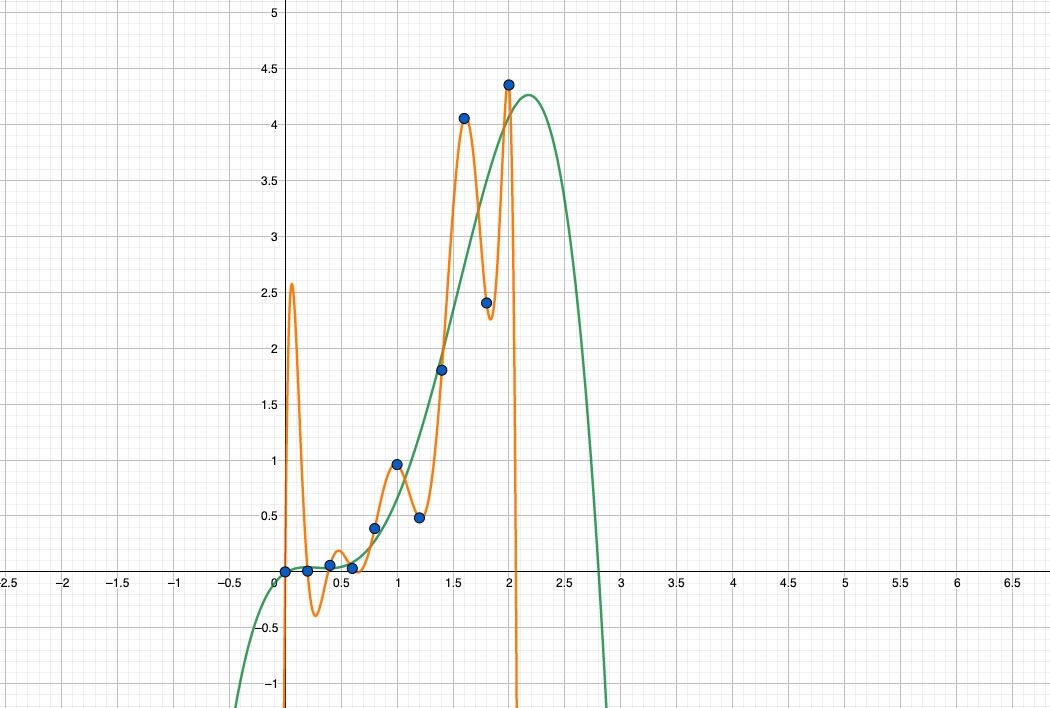
\includegraphics[width =\textwidth]{graphic}
Синие точки - точки, известные из условия \\
Оранжевая кривая - кривая интерполирующего многочлена в \\ форме Лагранжа \\
Зелёная кривая - кривая, построенная по методу наименьших квадратов

\section*{Анализ результатов}

\section*{Источники и ресурсы}
Вводные лекции по численным методам (Д.П. Костомаров, A.П. Фаворский) \\
Для построения графиков использовался ресурc \textit{www.geogebra.com}
\end{document}